\documentclass{beamer}

\usepackage[bulgarian]{babel}
\usepackage{amsfonts,amsmath}
\usepackage{lmodern}
\usepackage[notref,notcite]{showkeys}
\usepackage{graphicx}
\usepackage{wrapfig}

\newcommand{\RR}{\mathbb{R}}
\newcommand{\rf}[1]{(\ref{#1})}

\title{Числено решаване на двумерното стационарно парадигматично уравнение на Бузинеск}
\author{докторант: Красимир Ангелов 
\newline \newline научен ръководител: Наталия Кольковска}

\usetheme{default}
\begin{document}

%==================1======================================
\begin{frame}
\titlepage
\end{frame}


%==================2======================================
\begin{frame}
\frametitle{ Едномерното парадигматично уравнение на Бусинеск }
\begin{align}
&u_{tt} - u_{xx} -\beta_1  u_{ttxx} +\beta_2 u_{xxxx} + f(u)_{xx}=0   \quad \text{при} \,  x \in \RR, \, t\in\RR^+,\label{eq1D}
\\ \nonumber &u(x,0)=u_0(x), \, u_t(x,0)=u_1(x)   \quad\text{при} \, x \in \RR,
\\  &u(x) \rightarrow 0,  u(x)_{xx} \rightarrow 0 ,  \quad \text{при} \, x \rightarrow \infty, \label{eq1d1}
\end{align}
Точно решение от тип солитон при $u =\tilde u(x-ct)$:
\begin{align}
\tilde u(x,t:c) = \frac{3}{2} \frac{c^2-1}{\alpha}sech^2 \left( \frac{1}{2}  \sqrt{ \frac{\beta_1 (c^2-1)}{\beta_1 c^2-\beta_2}} (x-c t \sqrt{\frac{\beta_1}{\beta_2}} ) \right)
\end{align}
Солитона е самодвижеща се вълнова композиция, която запазва формата си, докато се разпространява с постоянна скорост. Структурата ѝ се запазва дори след взаимодействие с друг(и) солитон(и).
\end{frame}

%==================3======================================
\begin{frame}
\frametitle{ Двумерното $(x,y) \in \RR^2$ парадигматично уравнение на Бусинеск }
\begin{align}
&u_{tt} - \Delta u -\beta_1  \Delta u_{tt} +\beta_2 \Delta ^2 u + \Delta f(u)=0, \, t\in\RR^+,\label{eq1}
\\
&f(u) = u^2 \nonumber \\  \nonumber &u(x,y,0)=u_0(x,y), \, u_t(x,y,0)=u_1(x,y)  , 
\\  &u(x,y) \rightarrow 0, \,  \Delta u(x,y) \rightarrow 0 ,  \quad \text{при} \sqrt{x^2 + y^2} \rightarrow \infty, \label{eq11} 
\end{align}
\begin{itemize}
  \item Извеждане на {\color{red}стационарно} уравнение чрез полагането $U(x,y-ct)=u(x,y,t)$ в \rf{eq1}
\end{itemize}
\color{red}
\begin{equation}
c^2 (E_1-\beta_1 \Delta) U_{yy} = \Delta U -\beta_2 \Delta^2 U - \Delta f(U)
\end{equation}

\end{frame}

%==================3======================================
\begin{frame}
\frametitle{ Двумерното стационарно парадигматично уравнение на Бусинеск }

\begin{equation}\label{eq2}
c^2 (E_1-\beta_1 \Delta) U_{yy} = \Delta U -\beta_2 \Delta^2 U - \Delta f(U),
\end{equation}
Целта на настоящата работа е
\begin{itemize}
  \item да се намерят числени решения на \rf{eq2} при различни параметри $\beta$ и $c$ с висок ред на апроксимация - 2ри, 4ти и 6ти.
  \item да се намерят числени решения на \rf{eq2} за по-високи скорости близо до допустимия максимум $c \approx \min (1/ \sqrt{\beta_1},1)$, $c < \min (1/ \sqrt{\beta_1},1)$,
  \item да се построи ново гранично условие за  \rf{eq2}.
\end{itemize}
\end{frame}

%==================4======================================
\begin{frame}
\frametitle{Смяна на променливите, свойства на новото уравнение } 
 
\begin{itemize}
\item Смяната $x=\sqrt\beta_1 { \overline x}$, $y=\sqrt\beta_1 { \overline y}$, $U(x,y)= v({ \overline x},{ \overline y} )$ в елиптичното уравнение \rf{eq2} води до
 \begin{align}\label{eq3}
&c^2 \beta (E_1- \Delta) v_{{\overline y}{\overline y}} = \beta \Delta v - \Delta^2 v - \beta \Delta f(v), \\ 
&v(\overline x, \overline y) \rightarrow 0,  \Delta v(\overline x, \overline y) \rightarrow 0 ,  \quad \text{за}  \sqrt{\overline x^2 + \overline y^2} \rightarrow \infty, \nonumber
\end{align}
\end{itemize}
\begin{itemize}
  \item нов дисперсионен параметър $\beta := \beta_1/\beta_2$
  \item уравнение \rf{eq3} е елиптично (4ти ред) при $c < \min (1/ \sqrt{\beta},1)$
  \item преминаване към система от две уравнения - подобряване на устойчивостта
  \item скалиране на решението спрямо стойността $v(0,0)$ - търсят се ненулеви решения 
\end{itemize}

\end{frame}

%==================5======================================
\begin{frame}
\frametitle{Метод на простата итерация} 
\begin{itemize}
  \item C.I. Christov, Numerical implementation of the asymptotic boundary conditions for steadily propagating 2D solitons of Boussinesq type equations,
{\it Mathematics and Computers in Simulation}, \textbf{82} (2012), 1079-1092.
\end{itemize}

\begin{itemize}
  \item Въвеждат се две нови функции: $\widehat{v}=v/{\theta} $ и $\widehat{w}=w/{\theta} $, където $v(0,0)=\theta$
\end{itemize}
\begin{equation}\label{eq45}
\begin{split}
 &- (1 - c^2 \beta) \widehat{v}_{yy} -\widehat{v}_{xx} + \beta (1-c^2) \widehat{v} - \alpha \beta \theta \widehat{v}^2 = \widehat{w}, \\
 &- \Delta \widehat{w} =  c^2 \beta \widehat{v}_{xx}.
\end{split}
\end{equation}

\begin{itemize}
  \item Численото решение на системата \rf{eq45} се намира чрез метода на простата итерация като изкуствено се добавят производни по времето както следва:
\end{itemize}
\begin{align}\label{eq5}
\begin{split}
 &\frac {\partial \widehat{v}}{\partial t} - (1 - c^2 \beta) \widehat{v}_{yy} -\widehat{v}_{xx} + \beta (1-c^2) \widehat{v} - \alpha \beta \theta \widehat{v}^2 = \widehat{w}, \\
 &\frac {\partial \widehat{w}}{\partial t} - \Delta \widehat{w} =  c^2 \beta \widehat{v}_{xx}. 
\end{split}
\end{align}
%По този начин стационарната системата от двете уравнения \rf{eq45} се заменя с преходните във времето уравнения дефинирани в \rf{eq5} с условието, че решенията $\widehat{v}$ и $\widehat{w}$ схождат линейно спрямо времето към решенията на \rf{eq45}.



\end{frame}


%==================6======================================
\begin{frame}
\frametitle{Метод на простата итерация} 
Дискретизацията на последното уравнение \rf{eq5} води до следната явна схема:
\begin{equation}\label{eq555}
\begin{split}
\frac {\widehat{v}^{(k+1)}-\widehat{v}^{(k)}}{\tau}- (1-c^2 \beta) \widehat{v}^{(k)}  (\Delta_{h,p,s,y})^T - \quad\quad\quad\;&\\
-\Delta_{h,p,s,x}  \widehat{v}^{(k)}+ \beta (1-c^2 ) \widehat{v}^{(k)} - \beta \theta f(\widehat{v}^{(k)}) &= \widehat{w}^{(k)}, \\
\frac  {\widehat{w}^{(k+1)} -\widehat{w}^{(k)}} {\tau} - \Delta_{h,p,s,x}  \widehat{w}^{(k)} - \widehat{w}^{(k)}  (\Delta_{h,p,s,y})^T &=  c^2 \beta \Delta_{h,p,s,x}  \widehat{v}^{(k)}.
\end{split}
\end{equation}

Стойността на $\theta$ се намира използвайки следната зависимост
\begin{equation}\label{eqtheta}
\theta = \frac{ (1-c^2 \beta) \widehat{v}_{yy} + \widehat{v}_{xx} - \beta (1-c^2) \widehat{v} +\widehat{w}}{\alpha \beta \widehat{v}^2 } |_{x=0,y=0}.
\end{equation}
\end{frame}


%==================7.1======================================
\begin{frame}
\frametitle{Метод на простата итерация}

\begin{itemize}
  \item дискретизация - крайна област $\omega_h$ с размери $N_x \times N_y$
  \item матриците $\Delta_{h,p,s,x}$ и $\Delta_{h,p,s,y}$ имат една и съща структура, но различна големина.
  \item граничните условия са отразени със съответната точност и са включени в дефинираните по-долу матрици.
  \item диференчна схема от общ вид за оператора на Лаплас:
\begin{equation}\label{PsnDiscret}
-\Delta_{h,p,s}  V_h = -\Delta_{h,p,s,x}  V_h - V_h (\Delta_{h,p,s,y})^T = F_h,
\end{equation}
\begin{figure}
     \includegraphics[width=\linewidth]{FPSExplained.png}
	\label{fig:FPSexplained}
\end{figure}
\end{itemize}
Тук $V_h, F_h$ са двумерни матрици съответно с елементи  $v(x_i,y_j)$ и  $f(x_i,y_j)$ и големина $N_x\times N_y$. Дискретните функции $V_h, F_h$ представят непрекъснатите такива $v, f$ ограничени върху мрежата $\omega_h$, т.е. $V_h = v(\omega_h)$ и $F_h = f(\omega_h)$
\end{frame}

%==================7.2======================================
\begin{frame}
\frametitle{Метод на простата итерация}
\framesubtitle{Втори ред на апроксимация на вторите производни ($p=2$)}
Матриците $\Delta_{h,2,s,x}$ и $\Delta_{h,2,s,y}$ при $p=2$
\[
\frac{1}{h^2}
\begin{bmatrix}
    -2	       & 2        &     \dots   &   \dots        & 0   \\
    1               & -2            &   1           &   0               & \vdots    \\
        0           & \ddots        &    \ddots    &   \ddots       &  0 \\ 
    \vdots       &     0            &  1     	& -2    	   & 1 \\
    0               & \dots          &  \dots         & 1  	   & -2 \\
\end{bmatrix}
\]
\end{frame}

%==================8======================================
\begin{frame}
\frametitle{Метод на простата итерация}
\framesubtitle{Четвърти ред на апроксимация на вторите производни ($p=4$)}
Матриците $\Delta_{h,4,s,x}$ и $\Delta_{h,4,s,y}$ при $p=4$
\[
\Delta_{h,4,s,x} = \frac{1}{h^2}
\begin{bmatrix}
     -\frac{5}{2}	& \frac{8}{3}       & -\frac{1}{6}	&    0     			&    \dots      	   &   0           & 0    \\
    \frac{4}{3}          &-\frac{31}{12}    	& \frac{4}{3}	&   -\frac{1}{12}	  	&   \dots      	  &   0	           & \vdots  \\
    -\frac{1}{12}	& \frac{4}{3}         	& -\frac{5}{2}	&  \frac{4}{3}    	 &   -\frac{1}{12}	  &      0           &\vdots    \\
        0           		& \ddots        	&    \ddots   		 &   \ddots      	 &     \ddots      	  &  \ddots        &    0 \\	
\\
   \vdots      		 & 0           		 &  -\frac{1}{12}	& \frac{4}{3}    	& -\frac{5}{2}	&  \frac{4}{3}   &   -\frac{1}{12} \\
    0      		 &  \dots           	 &   0     		& -\frac{1}{12} 	 & \frac{4}{3} 	 & -\frac{5}{2}  &  \frac{4}{3}\\
    0              		 & \dots          	&  0              		 &\frac{1}{120} 	 &  -\frac{2}{15} 	& \frac{29}{20} & -\frac{38}{15}\\
\end{bmatrix}
\]
\end{frame}

%==================9======================================
\begin{frame}
\frametitle{Метод на простата итерация}
\framesubtitle{Шести ред на апроксимация на вторите производни ($p=6$) }
Матриците $\Delta_{h,6,s,x}$ и $\Delta_{h,6,s,y}$ при $p=6$
\[
\frac{1}{h^2}
\begin{bmatrix}
   -\frac{49}{18}		& \frac{3}{1}			&   -\frac{3}{10}		& \frac{1}{45}    		 &  0					& 0	   					&    0      	   	&   \dots           & 0    \\
    \frac{3}{2}    	&-\frac{517}{180}    	&    \frac{68}{45}     & -\frac{3}{20}  	 		& \frac{1}{90} 		&  0					 &   0      	   	&   \dots	       & \vdots  \\
    -\frac{3}{20}		& \frac{68}{45}         	& -\frac{49}{18} 	&  \frac{3}{2}		&  -\frac{3}{20}    	 &   \frac{1}{90}    	 &  0			&     \dots         &\vdots    \\
    \frac{1}{90}		& -\frac{3}{20}		& \frac{3}{2}         	& -\frac{49}{18} 	&  \frac{3}{2}		&  -\frac{3}{20}    	 &   \frac{1}{90} &     \dots         &\vdots    \\
        0           		& \ddots        		&         \ddots           	& \ddots        		&    \ddots   		&   \ddots      		 &     \ddots    	&  \ddots          &    0 \\	
\\
   \vdots      		&            		 	&    	0	      		& \frac{1}{90}		& -\frac{3}{20}		& \frac{3}{2}         	& -\frac{49}{18}	&  \frac{3}{2}  &  -\frac{3}{20} \\
    0      			&              	 	&    0      		&   -\frac{11}{11340}	 	&    \frac{2}{105} 	&  -\frac{5}{28} 	& \frac{884}{567} &-\frac{235}{84} &  \frac{54}{35}\\
    0              	& 	          		&    0              	&  -\frac{77}{13331}    		&  \frac{19}{420}&-\frac{1}{7}	 &  \frac{167}{1134} 	& \frac{191}{168}  &  -\frac{327}{140}\\
\end{bmatrix}
\]
\end{frame}

%==================10=====================================
\begin{frame}
\frametitle{Начални данни}
\begin{itemize}
  \item ``best-fit'' формули - Christov, C.I., Choudhury, J., Perturbation solution for the 2D Boussinesq equation, {\it Mech. Res. Commun.}, \textbf{38} (2011), 274-281,
  \item радиално симетрично решение при $c=0$ - Kolkovska N. Angelow K., Numerical computation of the critical energy constant for two-dimensional Boussinesq equations, {\it Application of Mathematics in Technical and Natural Sciences, Albena (Bulgaria)},
\emph{AIP Conference Proceedings}  \textbf{1684} (2015), 080007.
\end{itemize}


\end{frame}

%==================11=====================================
\begin{frame}
\frametitle{Контрол на стъпката по времето}

\begin{itemize}
  \item Когато $\tau > \tau_{stab}$ премине условието за устойчивост, решението започва да разхожда и да става негладко (назъбено)

  \item Тези знаци се проявяват първоначално при резидуала \rf{residual}, докато численото решение $u$ е все още монотонно

  \item Това е ясен знак, че стъпката $\tau$ трябва да се намали, в противен случай се увеличава.
\end{itemize}
Rезидуалът $R_{i,j}^{(k)}$ е дефиниран използвайки уравнение \rf{eq3}
\begin{align}\label{residual}
&R_{i,j}^{(k)} := 
c^2\beta (\widehat{v}^{(k)}_{i,j})_{\widehat{yy},p}  \nonumber \\
&+ \Delta_{h,p}(-\beta \widehat{v}^{(k)}_{i,j} - c^2\beta (\widehat{v}^{(k)}_{i,j})_{\widehat{yy},p} + \Delta_{h,p} \widehat{v}^{(k)}_{i,j} 
+ \alpha \beta \theta (\widehat{v}^{(k)}_{i,j})^2  ).
\end{align}

\end{frame}

%==================12=====================================
\begin{frame}
\frametitle{Критерии за спиране за уравнение \rf{eq555}}

Итеративният алгоритъм спира когато
\begin{itemize}
  \item разликата между две последователни решения стане достатъчно малка
	\begin{equation*}
	\Vert \widehat{v}^{(k+1)}-\widehat{v}^{(k)}\Vert  < \epsilon \Vert \widehat{v}^{(k)}\Vert ,
	\end{equation*}
\end{itemize}


\begin{itemize}
  \item резидуалът $R^{(k)}$ от \rf{residual} да изпълнява следната зависимост
	\begin{equation}\label{crit2}
	\max_{i,j} \Vert R_{i,j}^{(k)} \Vert < \epsilon,
	\end{equation}
\end{itemize}
при $L_\infty$ норма и достатъчно малък праг $\epsilon < 1\times10^{-9}$.

\end{frame}

%==================13=====================================
\begin{frame}
\frametitle{Ред на сходимост при Тест 1 - $\beta = 3$, $c=0.45$}

\begin{table}[ht]
\centering
		\begin{tabular}{||c|l|ll|ll||}
			\hline
			\hline
             & $h$  &  	$\Vert \bar{ E_i} \Vert_{L_2}$ 	& сход.	& $\Vert \bar{ E_i} \Vert_{L_\infty}$  		&сход.   \\
   					\hline 
					\hline 
$\beta = 3$   	&0.2    										&            &            &           &   \\
      c=0.45 	&0.1    & 0.014232  						&            & 0.016732 			&   \\
   $O(h^2)$     &0.05   & 0.003238  						&2.14  & 0.003997					& 2.07 \\
\hline 
$\beta = 3$   	&0.2   &            &            &             &    \\
      $c=0.45 $ &0.1   &   0.001758   &           &  0.002499  &   \\
       $O(h^4)$	&0.05  &  0.000114 & 3.95    & 0.000168  & 3.90  \\
\hline
$\beta = 3$   	&0.2   &            &        &                  &      \\
   $c=0.45$   	&0.1   &  0.005038 &           & 0.012462       &       \\
     $O(h^6)$	&0.05  &  0.000094  & 5.74  &  0.000323 & 5.27         \\
			\hline
			\hline 
		\end{tabular}
		\caption{Ред на сходимост при Метода на простата итерация с апроксимации $O(h^{2})$, $O(h^{4})$ и $O(h^{6})$ за Тест  1. Грешките $\bar{ E_i}$ са пресметнати в $L_2$ и $L_\infty$ норми.}
\label{tab:aA}
\end{table}

\end{frame}


%==================14=====================================
\begin{frame}
\frametitle{Ред на сходимост при Тест 2 - $\beta = 1$, $c=0.9$}

\begin{table}[ht]
\centering
		\begin{tabular}{||c|l|ll|ll||}
			\hline
			\hline
             & $h$  &  	$\Vert \bar{ E_i} \Vert_{L_2}$ 	& сход.	& $\Vert \bar{ E_i}\Vert_{L_\infty}$  		&сход.   \\
   					\hline 					
			\hline 	
$\beta = 1$   	&0.4   &             &           &                & \\
     $c=0.9$     &0.2   &  0.043898  &             & 0.017906      &    \\
     $O(h^2)$	&0.1  & 0.009999 & 2.13       & 0.004348      & 2.04  \\
\hline 	
 $\beta = 1$   	&0.4  &            &               &               &     \\
     $c=0.9$  	&0.2   & 0.006309  &              & 0.002965      &        \\
     $O(h^4)$	&0.1  &  0.000432 &3.87        & 0.000200 &  3.89        \\
    \hline
 $\beta = 1$	&0.4   &             &        &               &        \\
   $ c=0.9$  	&0.2   &  0.001423  &        & 0.000728      &       \\
       $O(h^6)$	&0.1  &   0.000121 &3.56  & 0.000015 &   5.57       \\
	   \hline
			\hline 
		\end{tabular}
		\caption{Ред на сходимост при Метода на простата итерация с апроксимации $O(h^{2})$, $O(h^{4})$ и $O(h^{6})$ и Тест 2. Грешките $\bar{ E_i}$ са пресметнати в $L_2$ и $L_\infty$ норми.}
\label{tab:aB}
\end{table}

\end{frame}

%==================14=====================================
\begin{frame}
\frametitle{Форма на решението}
\begin{figure}
	\begin{minipage}[b]{0.45\linewidth}
		\raggedleft
		\includegraphics[width=\linewidth]{../Thesis/SolutionProfiles/ChristovIVX=0_ZB2_bt1_c010_090_h020_O(h^6).png}
	\end{minipage}	
	\begin{minipage}[b]{0.45\linewidth}
		\raggedright
		 \includegraphics[width=\linewidth]{../Thesis/SolutionProfiles/ChristovIVY=0_ZB2_bt1_c010_090_h020_O(h^6).png}
	\end{minipage}
	\begin{minipage}[b]{0.45\linewidth}
		\raggedleft
		\includegraphics[width=\linewidth]{../Thesis/SolutionProfiles/ChristovIVLogX=0_ZB2_bt1_c010_090_h020_O(h^6).png}
	\end{minipage}	
	\begin{minipage}[b]{0.45\linewidth}
		\raggedright
		 \includegraphics[width=\linewidth]{../Thesis/SolutionProfiles/ChristovIVLogY=0_ZB2_bt1_c010_090_h020_O(h^6).png}
	\end{minipage}
	\label{profilesSpeedVarying}
\end{figure}

Сечения на численото решение по $x$ (ляво) и $y$ (дясно) осите при $\beta=1$ и различни скорости $c=0.1,0.3,0.5,0.7,0.9$. Горните картинки използват реални скали, а долните са изцяло логаритмични.
\end{frame}

%==================15=====================================
\begin{frame}
\frametitle{Форма на решението}
\begin{figure}[ht]
	\begin{minipage}[b]{0.45\linewidth}
		\raggedleft
		\includegraphics[width=\linewidth]{../Thesis/SolutionProfiles/ChristovIVX=0_ZB2_bt1_5_c017_h020_O(h^6).png}
	\end{minipage}	
	\begin{minipage}[b]{0.45\linewidth}
		\raggedright
		 \includegraphics[width=\linewidth]{../Thesis/SolutionProfiles/ChristovIVY=0_ZB2_bt1_5_c017_h020_O(h^6).png}
	\end{minipage}
	\begin{minipage}[b]{0.45\linewidth}
		\raggedleft
		\includegraphics[width=\linewidth]{../Thesis/SolutionProfiles/ChristovIVLogX=0_ZB2_bt1_5_c017_h020_O(h^6).png}
	\end{minipage}	
	\begin{minipage}[b]{0.45\linewidth}
		\raggedright
		 \includegraphics[width=\linewidth]{../Thesis/SolutionProfiles/ChristovIVLogY=0_ZB2_bt1_5_c017_h020_O(h^6).png}
	\end{minipage}
	\label{profilesDispVarying}
\end{figure}
Сечения на численото решение по $x$ (ляво) и $y$ (дясно) осите при $c=0.17$ и варираща дисперсия $\beta=1,2,3,4,5$. Горните картинки използват реални скали, а долните са изцяло логаритмични.
\end{frame}



%==================16=====================================
\begin{frame}
\frametitle{Форма на решението}
\begin{figure}[ht]
	\begin{minipage}[b]{0.45\linewidth}
		\raggedleft
		\includegraphics[width=\linewidth]{../Thesis/SolutionView/ChristovIC_30_bt3_c045_topview.png}
	\end{minipage}
	\begin{minipage}[b]{0.45\linewidth}
		\raggedright
		\includegraphics[width=\linewidth]{../Thesis/SolutionView/ChristovIC_128_bt1_c090_topview.png}
	\end{minipage}
	\begin{minipage}[b]{0.45\linewidth}
		 \raggedleft
		\includegraphics[width=\linewidth]{../Thesis/SolutionView/ChristovIC_30_bt3_c045_prpview.png}		
		\centerline{$\beta = 3$, $c = 0.45$ }
	\end{minipage}
	\begin{minipage}[b]{0.45\linewidth}
		 \raggedright
		\includegraphics[width=\linewidth]{../Thesis/SolutionView/ChristovIC_128_bt1_c090_prpview.png}
		\centerline{$\beta = 1$, $c = 0.9$}
	\end{minipage}
	\caption{2Д и 3Д профили на численото решение $\widehat v$ от \rf{eqtheta} и \rf{eq555}.}
	\label{fig:solutions}
\end{figure}

\end{frame}

%==================17=====================================
\begin{frame}
\frametitle{Сравнение с ``best-fit'' формулите}

Нека $D^*_{\kappa}$ да дефинира процентната разликата между двете решения  ``Метода на простата итерация'' $v$ и ``best-fit'' $v^*$ в ${L_2 }$ и ${L_\infty}$ норми, върху цялата област $\omega_h$:
\begin{equation}\label{diffvv}
D^*_{\kappa} := 100 \times \frac{\Vert v^*-v \Vert_{\kappa} }{ \Vert v \Vert_{\kappa} }.
\end{equation}
\end{frame}

%==================18=====================================
\begin{frame}
\frametitle{Сравнение с ``best-fit'' формулите}
\begin{table}[ht]
\centering
\begin{tabular}{|l|c|l l|l l|}
\hline 
\hline 
$\beta$	& c 	& $\|v^*-v \|_{L_2 }$ & $\|v^*-v \|_{L_\infty }$  	& $D^*_{L_2}$	& $D^*_{L_\infty }$	\\
\hline 
1& 		0.1	&	1.4772e-01 		& 	8.1024e-03 				& 2.7\%			& 1.7\%		\\
\hline 
1& 		0.3 	&	1.4310e-01 		& 	8.7770e-03				& 2.7\%			& 1.9\%		\\
\hline 
1& 		0.5 	&	1.6934e-01 		& 	1.3332e-02				& 3.5\%			& 3.3\%		\\
\hline 
1& 		0.7 	&	5.8673e-01		& 	5.1122e-02				& 14.8\%		& 16.2\%	\\
\hline 
1& 		0.9	&	2.1599e+0 		& 	1.6439e-01				& 93.1\%		& 121.2\%	\\
\hline 
\hline 
\end{tabular}
\caption{Разликите между числено решение $v$ получено с ``Метода на простата итерация'' и ``best-fit'' формулите $v^*$ при $\beta=1$ и $c=0.1, 0.3, 0.5, 0.7, 0.9$.}
\label{tab:diff-beta1}
\end{table}

\end{frame}

%==================19=====================================
\begin{frame}
\frametitle{Сравнение с ``best-fit'' формулите}
\begin{table}
\centering
\begin{tabular}{|l|c|l l| c|l|c|l l|}
\hline 
\hline 
$\beta$	& c 	& $\|v^*-v \|_{L_2 }$ & $\|v^*-v \|_{L_\infty }$  	& $D^*_{L_2}$	& $D^*_{L_\infty }$	\\
\hline 
1& 		0.17&	1.4704e-01 		& 	8.3793e-03 				& 2.7\%			& 1.8\%		\\
\hline 
2& 		0.17&	1.2688e-01 		& 	9.0013e-03				& 3.3\%			& 1.9\%		\\
\hline 
3& 		0.17&	1.3803e-01 		& 	1.3134e-02				& 4.4\%			& 2.8\%		\\
\hline 
4& 		0.17&	 1.5240e-01 		& 	1.7228e-02				& 5.7\%			& 3.7\%		\\
\hline 
5& 		0.17&	1.6720e-01 		& 	2.1844e-02				& 7.0\%			& 4.6\%		\\
\hline 
\hline 
\end{tabular}
\caption{Разликите между числено решение $v$ получено с ``Метода на простата итерация'' и ``best-fit'' формулите $v^*$ от \cite{Ch2011} при $\beta=1, 2, 3, 4, 5$ и $c=0.17$.}
\label{tab:diff-c017}
\end{table}
\end{frame}

%==================20=====================================
\begin{frame}
\frametitle{Извод на ново гранично условие}

\begin{itemize}
  \item  C.I. Christov,
Numerical implementation of the asymptotic boundary conditions for steadily propagating 2D solitons of Boussinesq type equations,
{\it Mathematics and Computers in Simulation}, \textbf{82} (2012), 1079-1092.
\begin{equation}
v(x,y) = v(r) ~ \frac{C_u}{r^2}, \quad r>>1
\end{equation}
  \item ново гранично условие
\begin{equation}\label{bndK}
\tilde v(x,y) = \mu_v \frac{ (1-c^2)x^2 - y^2}{ ((1-c^2)x^2 - y^2)^2}, \quad x^2 + y^2 >> 1.
\end{equation}
\end{itemize}
 

\end{frame}

%==================21=====================================
\begin{frame}
\frametitle{Асимптотично поведение на членовете от формула \rf{eq3}}
\begin{figure}
	\includegraphics[width=0.9\linewidth]{../Thesis/AssymptForEachTerm/c017_bt1_5/ChristovIC_AlongX_50_ZB2_bt1_c017_h020_O(h^6).png}
	\caption{Решението е получено с ``Метода на простата итерация'' и нулево гранично условие, $\boldsymbol{c=0.17}$ и $\boldsymbol{\beta = 1}$. }
	\label{fig:assympt_c017bt11}
\end{figure}

\end{frame}

%==================22=====================================
\begin{frame}
\frametitle{Асимптотично поведение на членовете от формула \rf{eq3}}
\begin{figure}
	\includegraphics[width=0.9\linewidth]{../Thesis/AssymptForEachTerm/c017_bt1_5/ChristovIC_AlongY_50_ZB2_bt1_c017_h020_O(h^6).png}
	\caption{ Решението е получено с ``Метода на простата итерация'' и нулево гранично условие, $\boldsymbol{c=0.17}$ и $\boldsymbol{\beta = 1}$. }
	\label{fig:assympt_c017bt12}
\end{figure}


\end{frame}

%==================23=====================================
\begin{frame}
\frametitle{Асимптотично поведение на членовете от уравнение \rf{eq3}}
Представените фигури в предишната част показват, че асимптотиката на членовете с производни от четвърти ред и нелинейните такива с производни от втори ред в \rf{eq3}
\begin{equation}\label{outliers}
- v_{xxxx}, \;  - (2-\beta c^2)v_{xxyy},  \;  - (1-\beta c^2)v_{yyyy}, \;  - \alpha \beta (v^2)_{xx}, \; - \alpha \beta (v^2)_{yy}
\end{equation}
e $O(r^{-6})$, а за останалите от втори ред
$$
\beta v_{xx}, \; \beta (1-c^2) v_{yy}
$$
асимптотиката е $O(r^{-4})$. Това дава основание да пренебрегнем членовете описани в \rf{outliers} от уравнение \rf{eq3} и да търсим точно решение на останалата част.
\end{frame}

%==================24=====================================
\begin{frame}
\frametitle{Извод на ново гранично условие}
Така за големи стойности на $r$, пренебрегвайки частите с по-нисък порядък $O(r^{-6})$, остават два водещи члена:
\begin{equation}\label{asymptEq}
\beta \tilde v_{xx} + \beta (1-c^2) \tilde v_{yy} =0, \quad \tilde v(x,y) \approx \frac{1}{x^2 + y^2}, \quad x^2 + y^2 >>1,
\end{equation}
взимайки предвид факта, че функцията $v(r)$ има асимптотика $O(r^{-2})$.

\end{frame}

%==================25=====================================
\begin{frame}
\frametitle{Извод на ново гранично условие}
\begin{itemize}
  \item  смяна на променливите $\bar x  = \sqrt{1-c^2} x$, $\bar y = y$ и $\tilde V (\bar x, \bar y)$ на променливите трансформира \rf{asymptEq} в уравнението на Лаплас
  \item преминаване в полярни координати $\bar \phi = arctan(\frac{\bar y}{\bar x})$, $\bar r = \sqrt{\bar x^2, \bar y^2}$ 
  \item разделяне на променливите $\tilde V_p(\bar r, \bar \phi) = H(\bar r) G(\bar \phi)$
\end{itemize}

\begin{align}\label{LaplaceSol}
&H(\bar{r}) = \sum^{\infty}_{n=0} (\mu_{1,n} \frac{1}{ \bar{r}^n} + \mu_{2,n} \bar{r}^n ),
\\ \nonumber &G(\bar \phi) = \sum^{\infty}_{n=0} (\mu_{3,n}sin(n \bar \phi ) + \mu_{4,n}cos(n \bar \phi)),
\end{align}
където $\mu_{1,n}, \mu_{2,n}, \mu_{3,n}, \mu_{4,n}, n \in \mathbb{N}_{0}$ са реални константи.

\end{frame}


%==================26=====================================
\begin{frame}
\frametitle{Извод на ново гранично условие}
\begin{itemize}
  \item решението има асимптотика от вида $1/r^2$, следователно
	\begin{equation}
	H(\bar r) = \mu_{1,2}\frac{1}{\bar r^2}, \quad \mu_{1,n} = 0, n \neq 2, \quad \mu_{2,n} = 0, n \ge 0
	\end{equation} 
  \item решението за достатъчно големи $r >> 1$ е положително върху абцисата и отрицателно върху ординатата, следователно
\begin{equation}
G(\bar \phi) = \mu_{4,2}cos(2 \bar \phi), \quad \mu_{3,n} = 0, n \ge 0, \quad \mu_{4,n} = 0, n \neq 2.
\end{equation}
  \item крайната формула за решението на \rf{asymptEq} в старите $(x, y)$ координати е еквивалентно на 
\begin{equation}\label{bndv}
\tilde v(x, y) = \mu_v \frac{ (1-c^2) x^2 - y^2 }{ ((1-c^2) x^2 + y^2)^2 }.
\end{equation}
\end{itemize}
\end{frame}

%==================27=====================================
\begin{frame}
\frametitle{Числени резултати получени с метода на простата итерация и новото гр. условие}
Числените експерименти показват, че при увеличаването на областта $\omega_h$; $L_x = L_y = 20, 40, 80, 160$
\begin{itemize}
  \item стойностите $\mu_v$ се установяват - абсолютната стойност от разликата между две последователни стойности намалява,
  \item разликите между численото решение $\widehat v$ и граничната функция $\tilde v$ в област близо до границата намалява измерено в $L_2$ норма,
  \item стойността на функцията $\widehat v(0,L_y)$ намалява с темп от вида $1/r^2$

\end{itemize}
\end{frame}

%==================28=====================================
\begin{frame}
\frametitle{Числени резултати получени с метода на простата итерация и новото гр. условие}
\begin{figure}[ht]
	\begin{minipage}[b]{0.45\linewidth}
		\raggedleft
		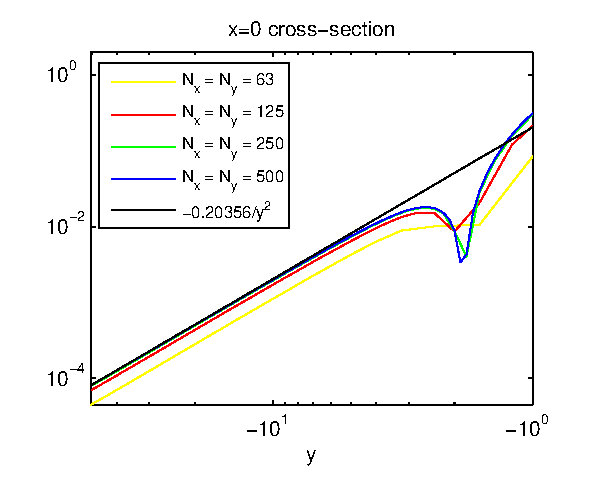
\includegraphics[width=\linewidth]{../Thesis/NewBoundaryCondition/crossSectionLogX=0.eps}
	\end{minipage}	
	\begin{minipage}[b]{0.45\linewidth}
		\raggedright
		 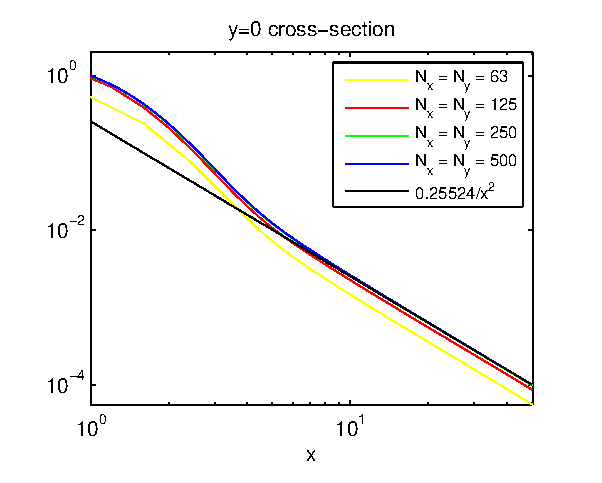
\includegraphics[width=\linewidth]{../Thesis/NewBoundaryCondition/crossSectionLogY=0.eps}
	\end{minipage}	
	\caption{Ефектът от промяната на дискретната стъпка по пространството $h=0.1, 0.2, 0.4, 0.8$. Показана е функцията $\widehat{v}$ в логаритмични скали по $x,\widehat v(x,0)$ и $y,\widehat v(0,y)$. }

\end{figure}
\end{frame}

%==================29=====================================
\begin{frame}
\frametitle{Числени резултати получени с метода на простата итерация и новото гр. условие}
\begin{figure}[ht]
	\begin{minipage}[b]{0.45\linewidth}
		\raggedleft
		\includegraphics[width=\linewidth]{../Thesis/NewBoundaryCondition/crossSectionX=0FF.eps}
	\end{minipage}	
	\begin{minipage}[b]{0.45\linewidth}
		\raggedright
		 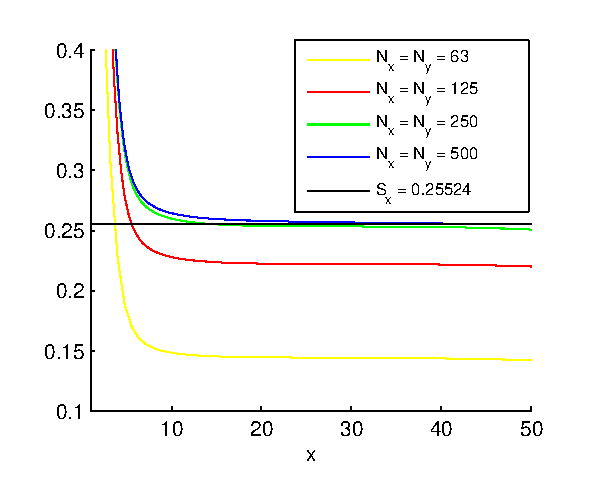
\includegraphics[width=\linewidth]{../Thesis/NewBoundaryCondition/crossSectionY=0FF.eps}
	\end{minipage}
	\caption{Ефектът от промяната на дискретната стъпка по пространството $h=0.1, 0.2, 0.4, 0.8$. На фигурите са описани следните криви: $(y, y^2 \widehat v(0,y)), \; (x, x^2 \widehat v(x,0))$. }
\end{figure}
\end{frame}


%==================30=====================================
\begin{frame}
\frametitle{Заключение}

\begin{itemize}
  \item Намерено е числено решение на стационарното уравнение на Бусинеск с висок ред на апроксимация $O(h^4)$ и $O(h^6)$
  \item така се намират нови числени решения за произволни параметри $\beta, c$ с условието, че $c < \min (1/ \sqrt{\beta},1)$
  \item направени са сравнения с ``best-fit'' формулите на проф. Христов,
  \item изведено е ново гранично условие
\end{itemize}

Това ни дава достатъчно знания, за да преминем към изследване на хиперболичната задача \rf{eq1} - \rf{eq11}
\end{frame}

\end{document}